
\begin{figure}[t]
\centering

\begin{subfigure}{0.32\linewidth}
\centering
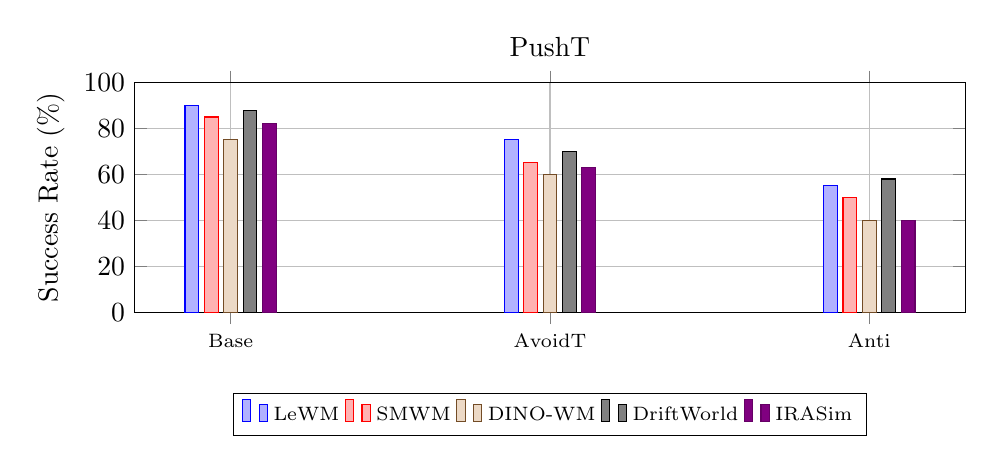
\begin{tikzpicture}
\begin{axis}[
    title={PushT},
    ybar,
    bar width=5pt,
    width=\linewidth,
    height=4.5cm,
    ymin=0,ymax=100,
    ylabel={Success Rate (\%)},
    symbolic x coords={Base,AvoidT,Anti},
    xtick=data,
    xticklabel style={font=\scriptsize},
    legend style={
        font=\scriptsize,
        at={(0.5,-0.35)},
        anchor=north,
        legend columns=5
    },
    enlarge x limits=0.15,
    grid=major,
]

\addplot coordinates {
(Base,90) (AvoidT,75) (Anti,55)
};
\addplot coordinates {
(Base,85) (AvoidT,65) (Anti,50)
};
\addplot coordinates {
(Base,75) (AvoidT,60) (Anti,40)
};
\addplot coordinates {
(Base,88) (AvoidT,70) (Anti,58)
};
\addplot coordinates {
(Base,82) (AvoidT,63) (Anti,40)
};

\legend{
LeWM,
SMWM,
DINO-WM,
DriftWorld,
IRASim
}

\end{axis}
\end{tikzpicture}
\end{subfigure}
%
\begin{subfigure}{0.32\linewidth}
\centering
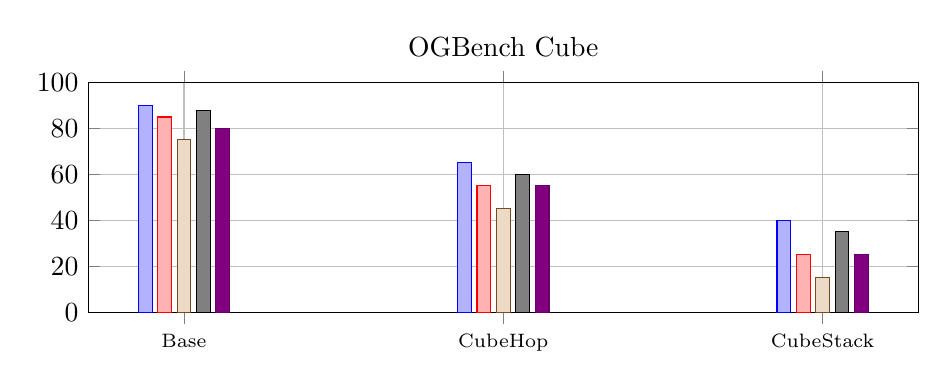
\begin{tikzpicture}
\begin{axis}[
    title={OGBench Cube},
    ybar,
    bar width=5pt,
    width=\linewidth,
    height=4.5cm,
    ymin=0,ymax=100,
    symbolic x coords={Base,CubeHop,CubeStack},
    xtick=data,
    xticklabel style={font=\scriptsize},
    enlarge x limits=0.15,
    grid=major,
]

\addplot coordinates {
(Base,90) (CubeHop,65) (CubeStack,40)
};
\addplot coordinates {
(Base,85) (CubeHop,55) (CubeStack,25)
};
\addplot coordinates {
(Base,75) (CubeHop,45) (CubeStack,15)
};
\addplot coordinates {
(Base,88) (CubeHop,60) (CubeStack,35)
};
\addplot coordinates {
(Base,80) (CubeHop,55) (CubeStack,25)
};

\end{axis}
\end{tikzpicture}
\end{subfigure}
%
\begin{subfigure}{0.32\linewidth}
\centering
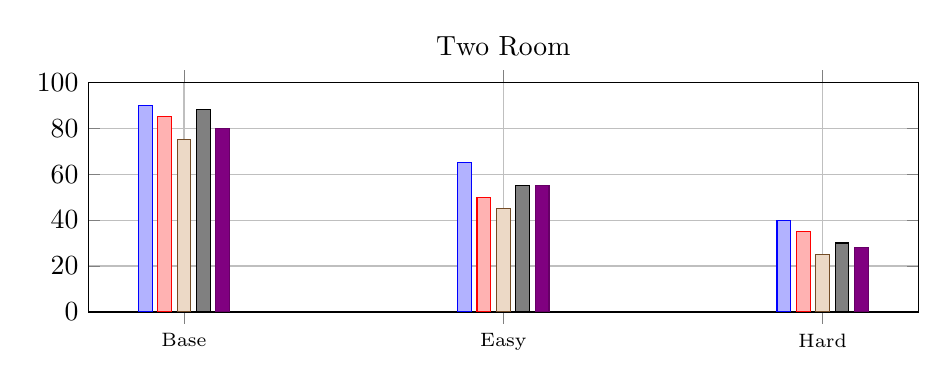
\begin{tikzpicture}
\begin{axis}[
    title={Two Room},
    ybar,
    bar width=5pt,
    width=\linewidth,
    height=4.5cm,
    ymin=0,ymax=100,
    symbolic x coords={Base,Easy,Hard},
    xtick=data,
    xticklabel style={font=\scriptsize},
    enlarge x limits=0.15,
    grid=major,
]

\addplot coordinates {
(Base,90) (Easy,65) (Hard,40)
};
\addplot coordinates {
(Base,85) (Easy,50) (Hard,35)
};
\addplot coordinates {
(Base,75) (Easy,45) (Hard,25)
};
\addplot coordinates {
(Base,88) (Easy,55) (Hard,30)
};
\addplot coordinates {
(Base,80) (Easy,55) (Hard,28)
};

\end{axis}
\end{tikzpicture}
\end{subfigure}

\caption{
MPC planning success rate of end-to-end world models.
Each environment family shows a consistent degradation from the base environment
to non-interactive and interaction-rich goal shifts.
}

\label{fig:e2e_planning}
\end{figure}